\documentclass[12pt,spanish,fleqn,openany,letterpaper,pagesize]{scrbook}

\usepackage[utf8]{inputenc}
\usepackage[spanish]{babel}
\usepackage{fancyhdr}
\usepackage{epsfig}
\usepackage{epic}
\usepackage{eepic}
\usepackage{amsmath}
\usepackage{threeparttable}
\usepackage{amscd}
\usepackage{here}
\usepackage{graphicx}
\usepackage{lscape}
\usepackage{tabularx}
\usepackage{subfigure}
\usepackage{longtable}


\usepackage{rotating} %Para rotar texto, objetos y tablas seite. No se ve en DVI solo en PS. Seite 328 Hundebuch
                        %se usa junto con \rotate, \sidewidestable ....


\renewcommand{\theequation}{\thechapter-\arabic{equation}}
\renewcommand{\thefigure}{\textbf{\thechapter-\arabic{figure}}}
\renewcommand{\thetable}{\textbf{\thechapter-\arabic{table}}}


\pagestyle{fancyplain}%\addtolength{\headwidth}{\marginparwidth}
\textheight22.5cm \topmargin0cm \textwidth16.5cm
\oddsidemargin0.5cm \evensidemargin-0.5cm%
\renewcommand{\chaptermark}[1]{\markboth{\thechapter\; #1}{}}
\renewcommand{\sectionmark}[1]{\markright{\thesection\; #1}}
\lhead[\fancyplain{}{\thepage}]{\fancyplain{}{\rightmark}}
\rhead[\fancyplain{}{\leftmark}]{\fancyplain{}{\thepage}}
\fancyfoot{}
\thispagestyle{fancy}%


\addtolength{\headwidth}{0cm}
\unitlength1mm %Define la unidad LE para Figuras
\mathindent0cm %Define la distancia de las formulas al texto,  fleqn las descentra
\marginparwidth0cm
\parindent0cm %Define la distancia de la primera linea de un parrafo a la margen

%Para tablas,  redefine el backschlash en tablas donde se define la posici\'{o}n del texto en las
%casillas (con \centering \raggedright o \raggedleft)
\newcommand{\PreserveBackslash}[1]{\let\temp=\\#1\let\\=\temp}
\let\PBS=\PreserveBackslash

%Espacio entre lineas
\renewcommand{\baselinestretch}{1.1}

%Neuer Befehl f\"{u}r die Tabelle Eigenschaften der Aktivkohlen
\newcommand{\arr}[1]{\raisebox{1.5ex}[0cm][0cm]{#1}}

%Neue Kommandos
\usepackage{Befehle}


%Trennungsliste
\hyphenation {Reaktor-ab-me-ssun-gen Gas-zu-sa-mmen-set-zung
Raum-gesch-win-dig-keit Durch-fluss Stick-stoff-gemisch
Ad-sorp-tions-tem-pe-ra-tur Klein-schmidt
Kohlen-stoff-Mole-kular-siebe Py-rolysat-aus-beu-te
Trans-port-vor-gan-ge}

\begin{document}

\justifying
\chapter{Modelando la Población del Vector de Dengue Utilizando Datos de Sensado Remoto y Aprendizaje Automático}

  \par Como mencionamos en capitulos anteriores, en un trabajo interinstitutional entre
    la Comisión Nacional de Actividades Espaciales (CONAE) y el ministerio de salud
    de Argentina, hubo iniciativas orientadas a modelar la evolución temporal de
    las poblaciones de mosquitos usando variables ambientales obtenidas de
    sensores remotos. Estos trabajos utilizaron series de algunos años y fueron
    basadas en un pequeño número de variables satelitales \cite{ndwi_erffectiveness, modis_data}.
    En un esfuerzo para mejorar esto, \cite{temporal_modeling}, construyeron modelos
    basados en una gran cantidad de variables de varios sensores de cuatro años.
    Aún así, todos estos trabajos asumieron modelos lineales multivariados.

  \par Este trabajo representa una mejoría sobre dicho escenario. Comparamos
    Support Vector Machines (SVM), Redes Neuronales Artificiales (ANN),
    K-vecinos más cercanos (KNN) y un tipo de árbol de decisión orientado a
    regresión, sumados a dos modelos de regresión lineal. Con ésto, se
    obtiene una metodología operaciónes que contribuye al sistema de riesgo
    de Dengue actualmente en operación \cite{porcasi_operative, analisis_cordoba}.

  \par Se explora, encontraste con los trabajos previos mencionados, la habilidad
    de modelado y predicción de oviposición con algoritmos de Aprendizaje
    Automático \textit{off-the-shelf}, i.e. algoritmos de software libre, ya
    implementados, sin mayores desarrollos sobre lo existente y con un ajuste de
    hyperparámetros minimo. De ésta manera se busca la asimilación de estas
    técnicas a toda la comunidad que se ocupa de problemas similares.


\section{Materiales}

\subsection{Datos de estudio y Datos de Campo}
  \begin{figure}
  \centering%
  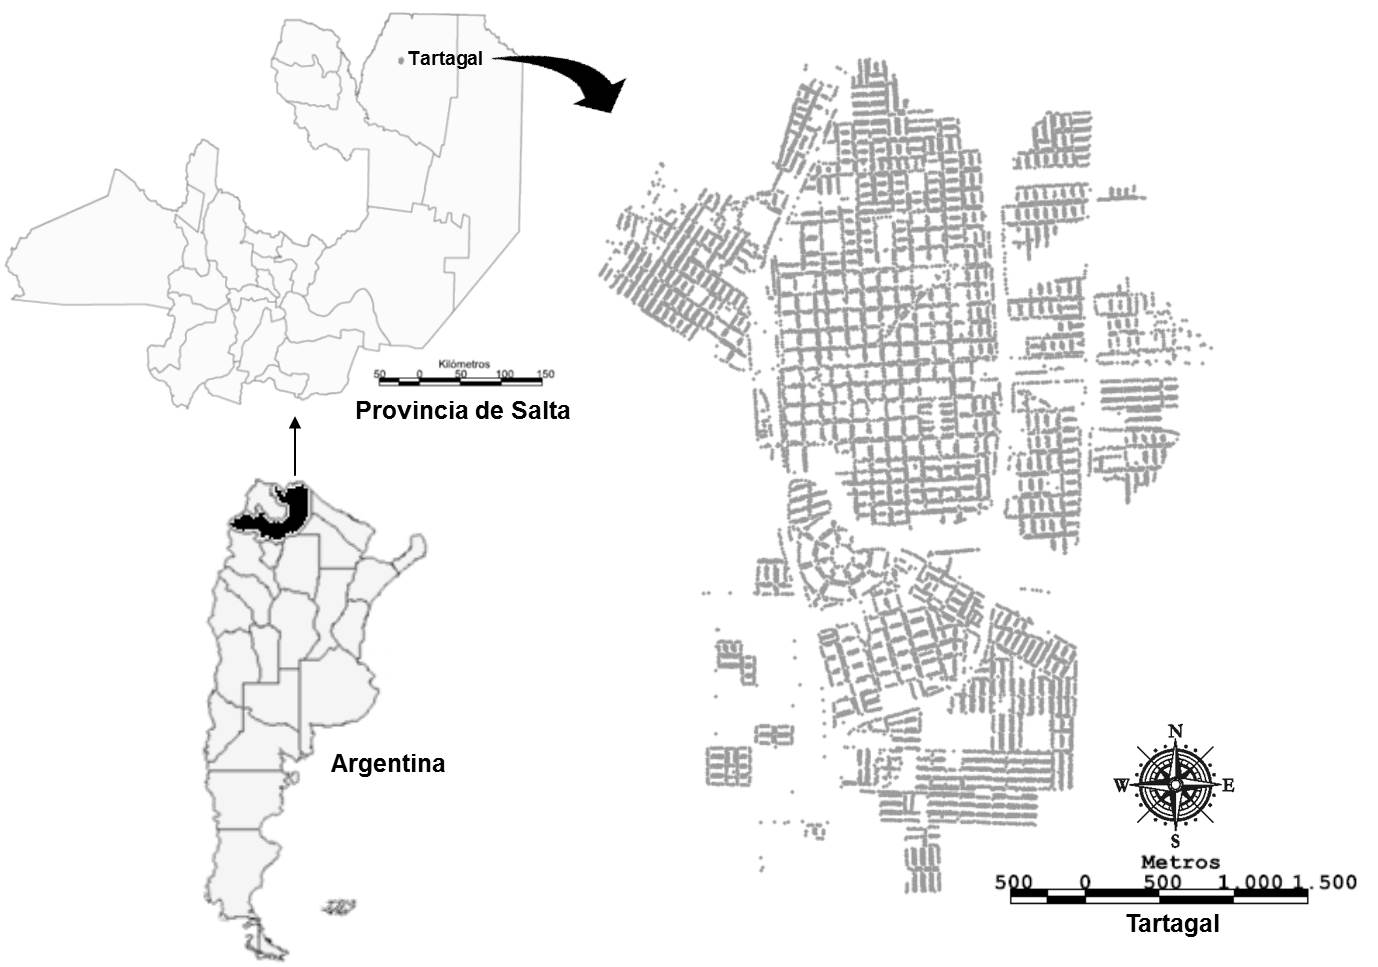
\includegraphics[width=0.6\textwidth]{images/tartagal}%
  \caption{Área de Estudio}\label{fig:tartagal}
  \end{figure}

  \par El estudio presentado fue desarrollado en la ciudad de Tartagal
    (con 79900 habitantes) en el noroeste de Argentina
    (\ang{22;32;}~S, \ang{63;49;}~O, \SI{450}{\meter} sobre el nivel del mar),
    en la provincia de Salta. El sitio está entre 50 y 100 kms de la frontera
    entre Argentina y Bolivia, como se puede apreciar en la Figura \ref{fig:tartagal}

  \par Este lugar tiene una temperatura media anual de unos \SI{23}{\degreeCelsius}
    (máximo promedio de verano de \SI{39}{\degreeCelsius} y minimo promedio en
    invieron de \SI{9}{\degreeCelsius}). Tiene una precipitación anual de
    \SI{1100}{\milli\meter}, con una estación seca (Junio a Octubre).
    Tartagal, como muchas ciudades del noroeste argentino, tiene una diversidad
    cultural basada en la presencia de grupos étnicos autóctonos y población
    de inmigrantes sumada al movimiento de migración proveniente de Bolivia.
    Estas características conducen a un perfil peculiar de comportamiento
    cultural, social y economico.

  \par La población de vectores es medida monitoreando la actividad de oviposición.
    Es medida usando ovitrampas colocadas en casas aleatoriamente seleccionadas
    en el área urbana de la ciudad. El período de monitoreo utilizado en este
    estudio fue de Agosto de 2012 hasta Julio de 2016 sobre 50 cassas. Dos
    ovitrampas fueron colocadas en cada una: una dentro y otra fuera de la casa,
    en el patio trasero en un lugar con sombra y a nivel del suelo, siguiendo
    las instrucciones de la OMS \cite{peridomestic}. Las ovitrampas son contenedores
    de \SI{1000}{\centi\meter\cubed} de plástico negro con \SI{250}{\milli\liter}
    de agua sin ninguna infusión de atracción.
    En este estudio sólo utilizamos los datos de las ovitrampas externas dado
    que ellas tienen una mayor correlación con las variables ambientales
    derivadas de información satelital. Dichas ovitrampas son reempazadas
    semanalmente y los huevos son contados en un laboratorio de acuerdo al
    \textit{Indice de Densidad de Huevos} \cite{indice_huevos}. Luego, la
    actividad de oviposición del \textit{Aedes Aegipty} es estimada por la suma
    de los huevos capturados en las trampas externas de la ciudad.



\subsection{Variables Ambientales}

  \par Siguiendo la idea de construir modelos predicticos de la población de
    vectores basados en variables ambientales derivadas de satelites, pero con una
    perspectiva operacional basada en trabajos previos, se obtuvieron representaciones
    de vegetación, humedad, temperatura y lluvia operacionalmente disponibles
    de \textbf{MODIS} y productos \textbf{TRMM/GPM}.

  \par Los índices de vegetación global proveen productos espaciales y
    temporales consistentes




\begin{center}
\begin{threeparttable}
\centering%
\caption{Participaci\'{o}n de las energ\'{\i}as renovables en el suministro
total de energ\'{\i}a primaria \cite{AG02i}.}\label{EMundo1}
\begin{tabular}{|l|c|c|}\hline
&\multicolumn{2}{c|}{Participaci\'{o}n en el suministro de energ\'{\i}a primaria /\% (Mtoe)\;$\tnote{1}$}\\\cline{2-3}%
\arr{Region}&Energ\'{\i}as renovables &Participaci\'{o}n de la biomasa\\\hline%
Latinoam\'{e}rica&28,9 (140)&62,4 (87,4)\\\hline%
\:Colombia&27,7 (7,6)&54,4 (4,1)\\\hline%
Alemania&3,8 (13,2)&65,8 (8,7)\\\hline%
Mundial&13,1 (1404,0)&79,4 (1114,8)\\\hline
\end{tabular}
\begin{tablenotes}
\item[1] \footnotesize{1 kg oe=10000 kcal=41,868 MJ}
\end{tablenotes}
\end{threeparttable}
\end{center}

\end{document}
